\chapter{引入预训练模型的联合识别}

事实证明,语言模型预训练对于学习通用语言表示很有用。 作为最新的语言模型预训练模型,BERT在许多语言理解任务中均取得了惊人的成绩,
使用双向transformer网络结构来预训练语言模型,着眼于单词左右两侧的上下文,具有更强的表达能力。可以通过附加输出层对bert进行微调来完成模型构建。
在本章,我们希望最大程度的利用bert预训练学到的语义编码能力,来提升第三章中提到的模型的准确率。

\section{算法描述}
向量编解码

\section{服务分类、接口分类与参数填充联合识别}
\subsection{单向联合}
考虑到参数提取任务和服务分类、接口分类任务之间存在很强的关系,本节进行了联合识别的尝试,以便通过全局优化获得更好的语义理解结果。
pipeline方法(上一章)通常是各自独立的模块,因此提出了联合模型,以期通过多个任务之间的相互增强来改善句子级语义理解结果。同时,和上一章
一样,注意力机制被引入并引入到模型中,以提供精确的焦点。
联合损失函数的方法“隐式”考量了这三个任务之间的联系,但并未明确为服务分类,接口分类和服务参数填充之间的进行关系建模,
考虑到由于服务参数填充通常高度依赖于前两个任务,
因此本节的模型着重于如何通过引入时隙门控机制来对服务分类,接口分类和服务参数填充之间进行显式关系建模。

\begin{figure}[htbp]
    \centering
    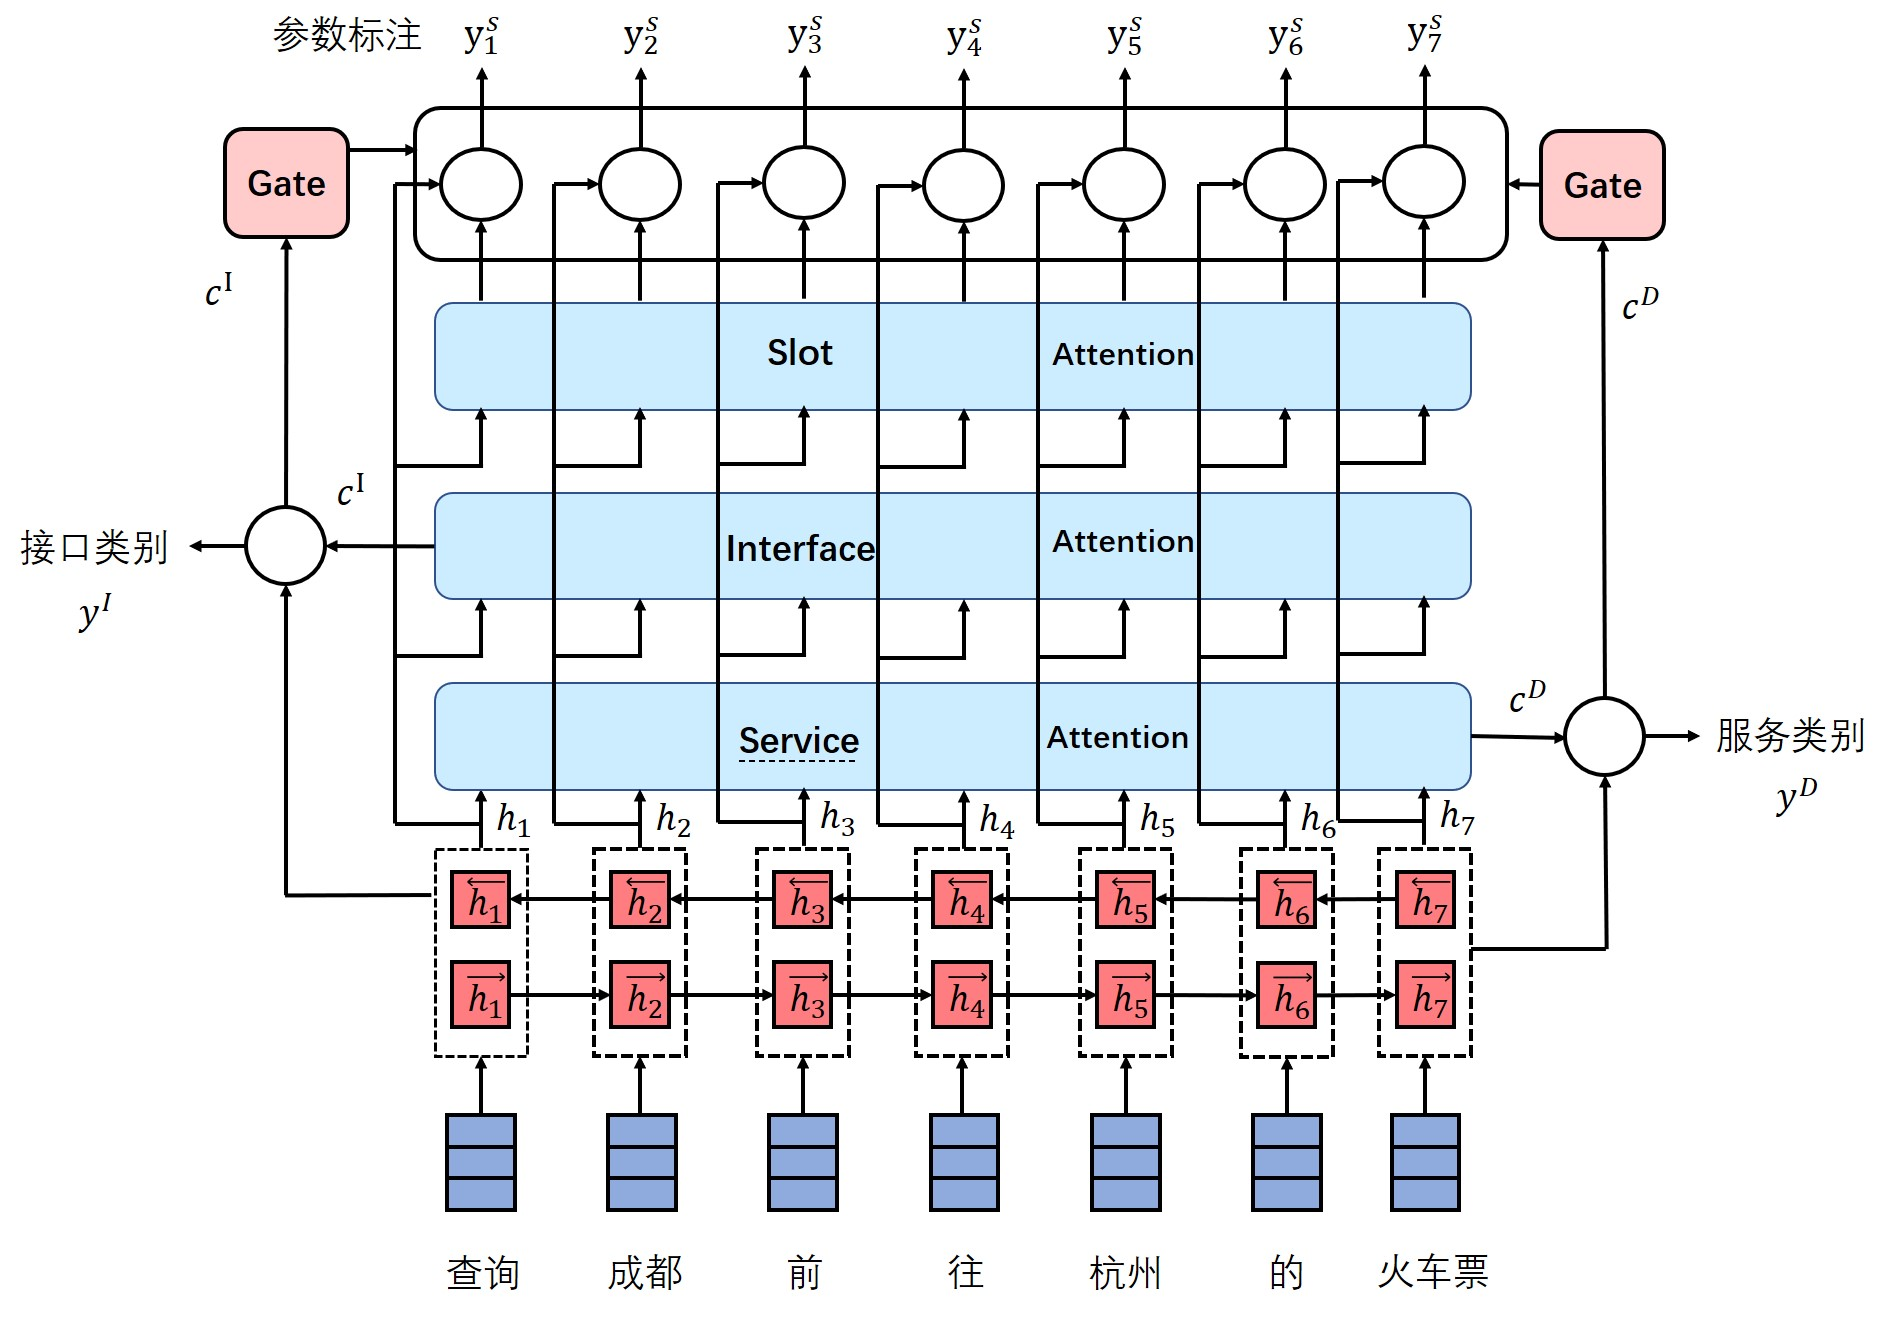
\includegraphics[width=17cm]{./images/lianhe.jpg}
    \caption{联合识别模型}
    \label{fig:lianhe1}
  \end{figure}

如图\ref{fig:lianhe}所示,是我们选择的联合识别模型。我们假设输入的词序列是x=[$x_{1}$,$x_{2}$,\dots,$x_{T}$],$x_{i}$经过双向LSTM处理后
得到的结果是$\overleftarrow{\mathbf{h}}_{i}$和$\overrightarrow{\mathbf{h}}_{i}$,拼接以后在第i步得到的结果是$\mathbf{h}_{i}=[\overrightarrow{\mathbf{h}}_{i} ;\overleftarrow{\mathbf{h}}_{i}]$。
1)三个attention层的计算方式

我们在联合模型中共设置了三层注意力机制,分别用于对应服务分类、接口分类与参数填充,三者的attention原理相同,只是会训练各自的参数,因此可以合并介绍。
设BLSTM得到的隐层向量序列为$h_{1}$,$h_{2}$,\dots,$h_{T}$,我们引入上下文向量${c}_{i}$来表示经过attention权重$α_{i,j}$和处理后的BLSTM隐层向量,
具体的${c}_{i}^{D}$,${c}_{i}^{I}$,${c}_{i}^{S}$分别表示用于服务分类、接口分类与参数填充任务的上下文向量:
\begin{equation}
    \mathbf{c}_{i}=\sum_{j=1}^{T} \alpha_{i, j} \mathbf{h}_{j}
  \end{equation}
  其中$\alpha_{i, j}$也根据所在具体的attention层不同分为$\alpha_{i, j}^{D}$,$\alpha_{i, j}^{I}$,$\alpha_{i, j}^{S}$,计算公式如下:
  \begin{equation}
    \alpha_{t, j}=\frac{\exp \left(\operatorname{score}\left(\mathbf{h}_{i}, \mathbf{h}_{j}\right)\right)}{\sum_{k} \exp \left(\operatorname{score}\left(\mathbf{h}_{i}, \mathbf{x}_{k}\right)\right)}
    \end{equation}
    \begin{equation}
      \operatorname{score}(\mathbf{h}_{i}, \mathbf{h}_{j}))=\tanh \left(\mathbf{W}\left[\mathbf{h}_{i} ; \mathbf{h}_{j}\right]\right)
    \end{equation}
显然这里的$\mathbf{W}$可由任务具体分为$\mathbf{W}_D$,$\mathbf{W}_I$,$\mathbf{W}_S$

2)服务分类

我们以1)中计算服务分类上下文向量的方法可以得到${c}_{i}^{D}$,再从BLSTM中取$\overleftarrow{\mathbf{h}}_{1}$和$\overrightarrow{\mathbf{h}}_{T}$,
$c^{D}$表示所有步骤得到的$c_i^{D}$的均值,服务的分类预测可由下式得到:
\begin{equation}
    y^{D}=\operatorname{softmax}\left(W^{D}\left(\overleftarrow{\mathbf{h}}_{1}+\overrightarrow{\mathbf{h}}_{T}+c^{D}\right)\right)
  \end{equation}
  \begin{equation}
    c^{D}=\frac{\sum_{i=1}^{T} c_i^{D}}{T}
  \end{equation}
3)接口分类

  我们以1)中计算接口分类上下文向量的方法可以得到${c}_{i}^{D}$,再从BLSTM中取$\overleftarrow{\mathbf{h}}_{1}$和$\overrightarrow{\mathbf{h}}_{T}$,
  $c^{I}$表示所有步骤得到的$c_i^{I}$的均值,服务的分类预测可由下式得到:
  \begin{equation}
      y^{I}=\operatorname{softmax}\left(W^{I}\left(\overleftarrow{\mathbf{h}}_{1}+\overrightarrow{\mathbf{h}}_{T}+c^{I}\right)\right)
    \end{equation} 
    \begin{equation}
        c^{I}=\frac{\sum_{i=1}^{T} c_i^{I}}{T}
      \end{equation}

      \begin{figure}[htbp]
        \centering
        
\includegraphics[scale=0.5]{./images/gate.jpg}
        \caption{gate结构}
        \label{fig:gate}
      \end{figure}

4)参数填充

如图\ref{fig:lianhe}中的gate,我们引入槽填充的控制门利用服务类型上下文向量${c}_{i}^{D}$和接口类型上下文向量${c}_{i}^{I}$来建立服务、接口与参数填充的关系
期望提高槽填充的准确率。${c}^{D}$,${c}^{I}$,${c}_{i}^{S}$会在每一个步长传入gate\ref{fig:gate}门结构中计算:
\begin{equation}
    g=\sum v \cdot \tanh (c_{i}^{S}+W_D \cdot c^{D}+W_I \cdot c^{I})
  \end{equation}
其中$\mathbf{v},\mathbf{W}_D,\mathbf{W}_I$是可训练的参数,数值g可以被看作联合上下文向量${c}^{D}$,${c}^{I}$,${c}_{i}^{S}$计算得到的权值,
较大的g表示slot上下文向量和D、I上下文向量注意到了输入序列的同一部分,可以推断出该语义槽和服务、接口之间的相关性更强,更有可能为我们需要提取的参数。
最终第i个词的标签类别信息可由下式计算得出:
\begin{equation}
    y_{i}^{S}=\operatorname{softmax}\left(W_{h y}^{S}\left(h_{i}+c_{i}^{S} \cdot g\right)\right)
  \end{equation}

5)联合目标函数
为了同时完成服务分类、接口分类与参数填充三项任务,需要建立联合损失函数,假设$y^D,y^I,y^S$表示正确的类别与标注,我们的目标
便是使在输入为$\mathbf{x}$的条件下概率$p\left(y^{S}, y^{I},y^{D} \mid \mathbf{x}\right)$最大:
\begin{equation}
    \begin{array}{l}
        p\left(y^{S}, y^{I},y^{D} \mid \mathbf{x}\right) \\
        =p\left(y^{D} \mid \mathbf{x}\right) p\left(y^{I} \mid \mathbf{x}\right) \prod_{t=1}^{T} p\left(y_{t}^{S} \mid \mathbf{x}\right) \\
        =p(y^{D} \mid x_{1}, \ldots, x_{T}) p(y^{I} \mid x_{1}, \ldots, x_{T}) \prod_{t=1}^{T} p(y_{t}^{S} \mid x_{1}, \ldots, x_{T})
        \end{array}
    \end{equation}

\subsection{交互式联合}
上一个的模型完成了从各任务独自建模到服务分类、接口分类向参数填充传递信息流的转换,但我们希望在任务与任务之间能够建立双向的信息交互。
直观的讲,如果用户的意图是调用平台内部的火车票查询服务,他输入的语句更可能出现诸如起始终点城市,日期等语义槽;反之,如果一句话中包含了
出发的起始,目的地和日期,那用户的意图更可能是调用行程相关的服务。因此,考虑到两个任务之间的交叉影响十分重要。


\section{结合bert的模型}

\section{结合ernie的模型}

